\documentclass[]{standalone}
\usepackage{luatexja}
\usepackage{tikz}

\tikzstyle{listNode}=[
  draw,
  thin,
  rectangle,
  minimum width = 2cm,
  text centered,
  minimum height = 1cm
]

\begin{document}
  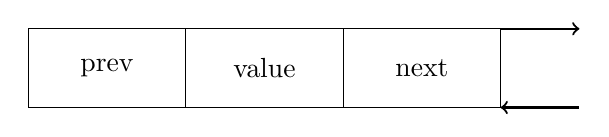
\begin{tikzpicture}
    \node[listNode] at (0,1) {prev};
    \node[listNode] at (2,1) {value};
    \node[listNode] at (4,1) {next};
    \draw[thick,->] (5,1.5) -- (6,1.5);
    \draw[thick,<-] (5,0.5) -- (6,0.5);
  \end{tikzpicture}

  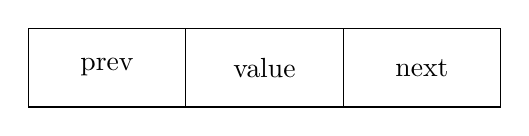
\begin{tikzpicture}
    \node[listNode] at (0,1) {prev};
    \node[listNode] at (2,1) {value};
    \node[listNode] at (4,1) {next};
  \end{tikzpicture}
\end{document}
